\chapter{Implementation of Privacy Protection Measures}
\section{Privacy Policy} \label{sec:PP}

In complience legal requirements of the Data Protection Directive (cf. Section \ref{EUDIR}) we include the following
Privacy Policy on our Mobile Application and Website.

\begin{quote}
\tt \small
\textbf{Privacy Policy}\\
==============

\textbf{What Personal Information do we Collect?}\\
The Mobile Sensor Collection Application collects the following data from your mobile phone:\\
- Sensor Data from Accelerometer\\
- Sensor Data from GPS sensors\\
- Daily Human Activities (walking, standing, sitting, etc.)\\
- Used Service Lines (bus, train, tram)

All collected data is transferred to our data center. The Live+Gov
Services does NOT store or collect names and email addresses.

\textbf{Which processing is applied to the data?}\\
We process Accelerometer samples on the Mobile device in order to extract human activities.
We process GPS coordinates on the Live+Gov server to extract the currently used service lines.

The stored information is used to produce aggregate reports.
These reports are based on anonymized data that do not allow the reconstruction of the routes of individual persons at a given point in time.

\textbf{Access to Stored Data}\\
All personal data can be accessed at our Privacy Dashboard at
\url{http://liveandgov.uni-koblenz.de/trial/dashboard}

There you have the possibility to:\\
- View all recordings made\\
- Delete individual recordings\\
- View the raw data collected for each recording\\
- Download the data for each recording\\
- View the results of the applied data processing

\textbf{When is the data deleted?}\\
The full data-set will be stored until January 2016.

Anonymized artifacts of this data are stored longer than that and will
be used by the Consortium Partners for research purposes.

\textbf{For which purposes is the data collected?}\\
The collected data will be used for personalization of user experience
of the mobile application.  Moreover, we will analyze travel patterns
in the Helsinki Urban region for general research and for improvement
and optimization of the infrastructure provided by HSL.

\textbf{Collaboration with Third Parties}\\
The raw data is not shared with any parties external to the Live+Gov
Consortium.

\textbf{Who has access to the data?}
The following organizations inside the Live+Gov Consortium have access
to the collected data:
\begin{enumerate}
\item University of Koblenz-Landau
\url{http://www.uni-koblenz-landau.de/}\\
Universitätsstraße 1\\
56070 Koblenz

\item Mattersoft \\
\url{http://www.mattersoft.fi/} \\
Hämeenkatu 13, 33100 Tampere, Finland\\
+358 10 3225000

\item Centre for Research and Technology Hellas (CERTH)\\
\url{http://mklab.iti.gr/contact}\\
6th km Charilaou-Thermi Road\\
P.O. Box 60361,\\
57001 Thermi-Thessaloniki, Greece
\end{enumerate}

Aggregated report based on anonymized data are disclosed to officials
at HSL \url{http://www.hsl.fi/} and might be made public in the form
of a blog post or research article.  These aggregated reports show
distributions of all routes that have been collected in the system and
do not allow to infere the location of a single user at a given point
in time.

\textbf{Identity of Data Controller}\\
The data is controlled by Dr. H.  Hartmann <hartmann@uni-koblenz.de>.

\textbf{Consent}\\
I have read and understood the above privacy policy and agree that my data is collected and processed accordingly.
\end{quote}

\section{Privacy Dashboard}
The Live+Gov Privacy Dashboard is a software component that allows the
citizens to view and control the data about themselves that is stored
in the Sensor Data Storage server.  The foundation of the Privacy
Dashboard component is the inspection tool that was introduced in D1.1
as a means to perform basic quality controlling of the collected data.

The Privacy Dashboard is currently endowed with the following views:
\begin{itemize}
  \item \textbf{Login Screen} (cf. Figure \ref{fig:PDLogin}).  Before
    access to the dashboard is granted, the user is prompted for
    credentials.  The credentials are generated by the sensor
    collection application on the mobile device.  The username can be
    freely chosen by the user. The password is then generated by the
    mobile application and transferred to the server alongside with
    the recording.

 \item \textbf{Recording Overview} (Cf. Figure \ref{fig:PDOverview}).
   This view shows all recordings that the user submitted to the Data
   Storage Service including basic meta information like start data of
   recording, duration. The user can click on each recording in order
   to view the recorded data in the Raw Data View.

   An important feature of the recording overview table is the delete
   button (cross on the very left.) That allows the user to
   selectively delete recordings, that shall not be analyzed by the
   Live+Gov system. Internally the click on the delete button only
   flags the corresponding trip for deletion. The actual deletion is
   carried out as a batch job on a regular bases. This addition step
   prevents accidental loss of data.

 \item \textbf{Raw Data View} (cf. Figure \ref{fig:PDRawData}).
   The raw data view shows all recorded raw data to the user.  GPS
   data is visualized on a map. Motion sensor data is displayed as
   plots. Wifi and GSM data is displayed in lists.  The raw data from
   each sensor can be downloaded individually as CSV file.

 \item \textbf{Processing View} (cf. Figure \ref{fig:PDProcessedData}).
   The processing view shows the data mining end-products for each
   processing step.  The Figure shows the processing view for the
   Activity Recognition. On the top a time-line is show that
   visualizes the different recognized activities via color-coding. A
   map below displays the corresponding GPS track with the same color
   coding.

   A similar view for Service Line Detection results is currently
   under development.
 \item \textbf{Privacy Settings.}
   This view contains the privacy policy shown in Section \ref{sec:PP}.

   We intend to include settings also settings concerning the
   expiration date of the recordings, agreements to certain processing
   steps, view logs of performed processing.
\end{itemize}

The Privacy Dashboard is implemented on a
nodes.js\footnote{\url{http://nodejs.org}} web server using
Express.js\footnote{\url{http://expressjs.com/}} as a web-framework
and d3.js\footnote{\url{http://d3js.org/}} as plotting library. The
data is pulled directly from the PostgreSQL database of the Data
Storage Service.

\begin{figure}
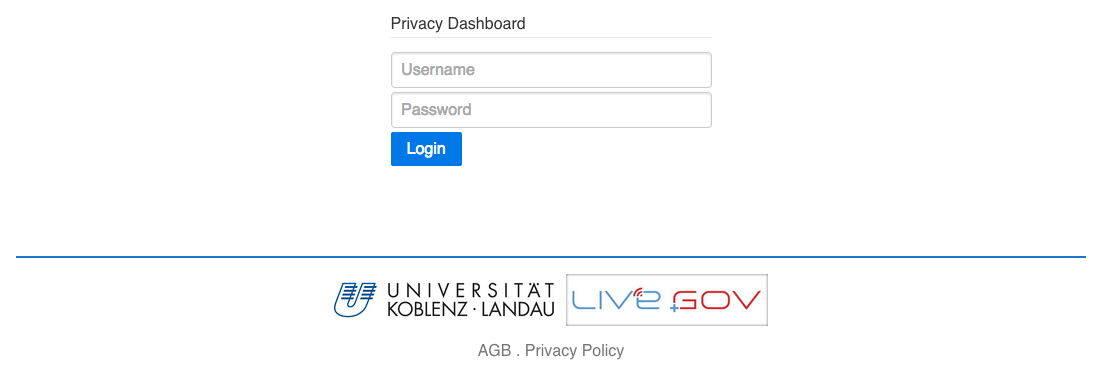
\includegraphics[width=\textwidth]{screenshots/login.png}
\caption{Live+Gov Privacy Dashboard Login}
\label{fig:PDLogin}
\end{figure}

\begin{figure}
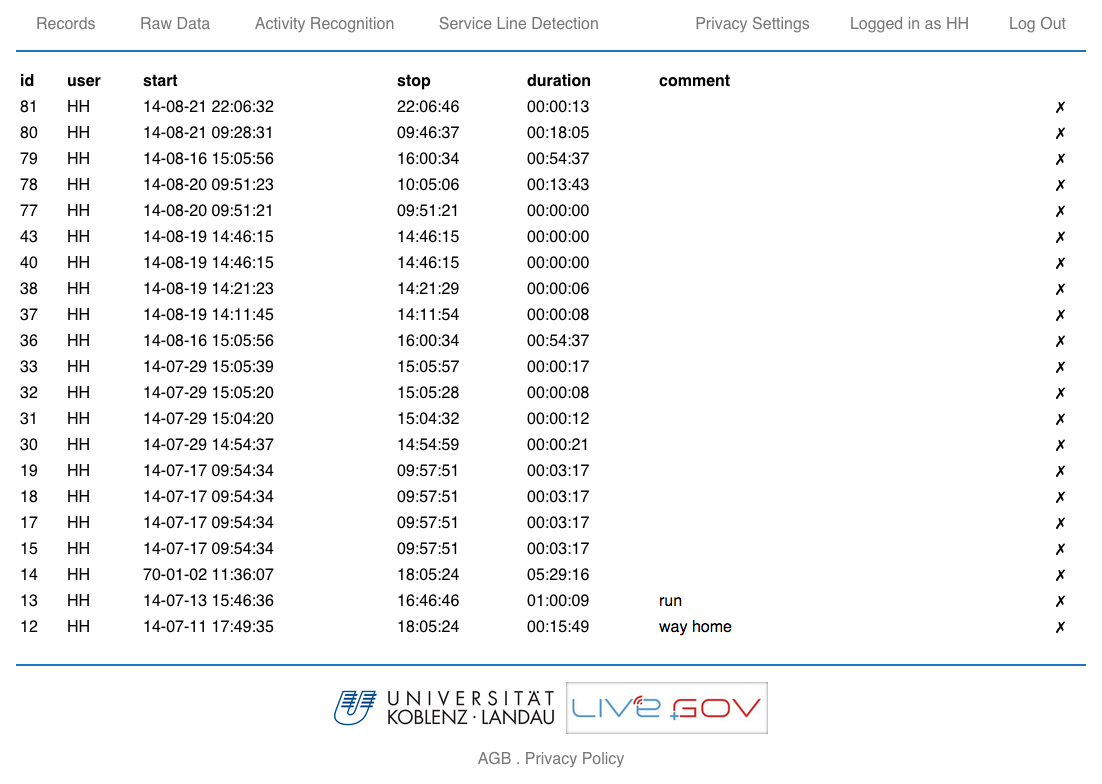
\includegraphics[width=\textwidth]{screenshots/recordings.png}
\caption{Live+Gov Privacy Dashboard Recording Overview}
\label{fig:PDOverview}
\end{figure}

\begin{figure}
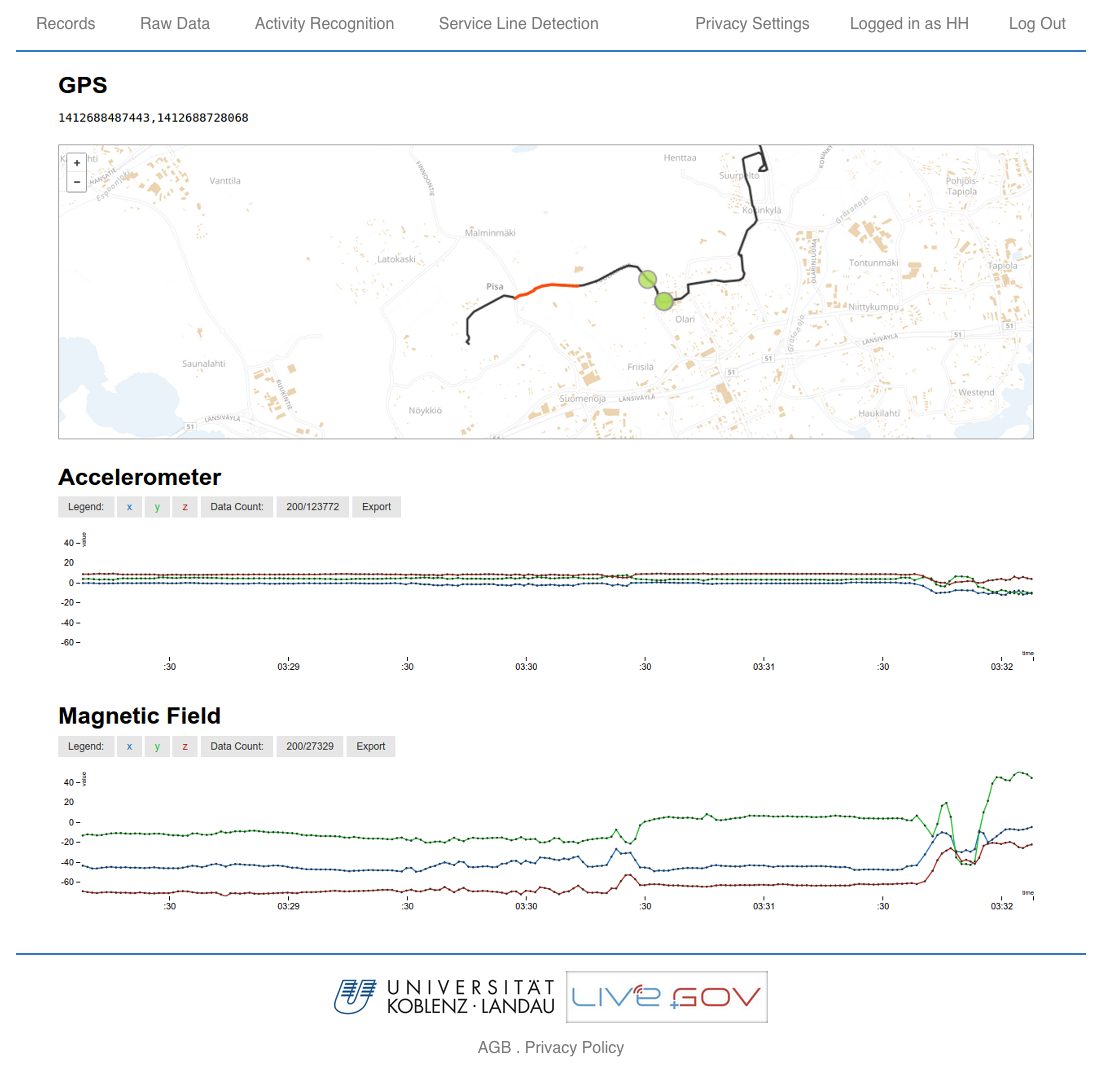
\includegraphics[width=\textwidth]{screenshots/raw.png}
\caption{Live+Gov Privacy Dashboard Raw Data View}
\label{fig:PDRawData}
\end{figure}

\begin{figure}
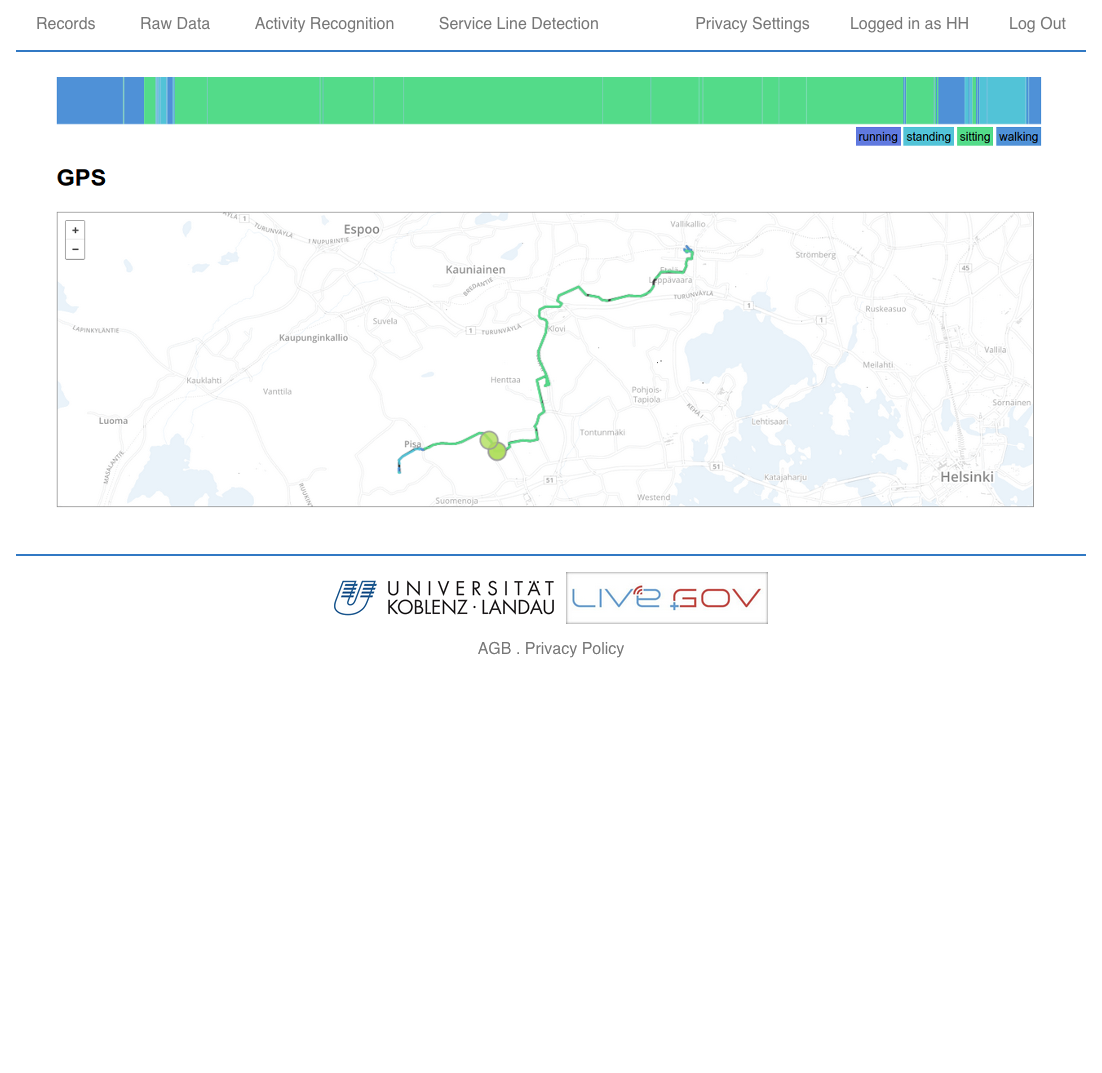
\includegraphics[width=\textwidth]{screenshots/processed.png}
\caption{Live+Gov Privacy Dashboard Processed Data View}
\label{fig:PDProcessedData}
\end{figure}

\pagebreak

\section{Transfer Encryption (HTTPS/SSL)}
The data transfer from the mobile device to the Data Storage component
as well as the transfer to the Privacy Dashboard relay on HTTP. In
order to avoid eavesdropping by externals that have access to the
communication channels, we secured all HTTP connections with SSL
encryption.

The implementation of this measure was rather straight forward. A SSL
certificate was issued by the University of Koblenz, and installed to
our webservers. Requests to this servers can now be done using HTTPS.
Figure \ref{fig:PDHTTPS} shows a screenshot of such a secured
connection to our Privacy Dashboard. The necessary adjustments to the
Sensor Collection Component were minimal, since Android comes with
native support for HTTPS connections.

\begin{figure}[h]
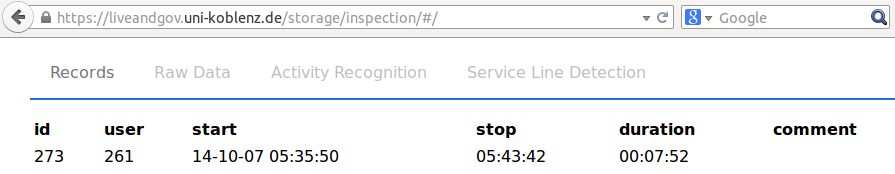
\includegraphics[width=\textwidth]{screenshots/HTTPS.png}
\caption{HTTPS connection to Privacy Dashboard}
\label{fig:PDHTTPS}
\end{figure}

\section{Data Expiring Dates}
Trips stored in the Sensor Data Storage Service have been endowed with
a data expiration date. A python script is provided that performs the
of expired data. In our installation we have this script running as a
cron job every night. The resulting schema of the trip table listed in
Figure \ref{fig:TripScheme}. The expiring date is encoded as a 64bit
integer holding the unix timestamp in seconds of the expiration date.

By default the expiration data is set to one year after the recording
was uploaded. We are working on including a feature for setting the
expiration date for each recording inside the privacy dashboard.

\begin{figure}
\begin{center}
\begin{alltt}
  Column  |          Type
----------+------------------------
 trip_id  | integer
 user_id  | character varying(36)
 start_ts | bigint
 stop_ts  | bigint
 name     | character varying(255)
 deleted  | boolean
 \textbf{expires}  | \textbf{bigint}
\end{alltt}
\end{center}
\caption{Database Schema of the Trip Table}
\label{fig:TripScheme}
\end{figure}

\section{Anonymization of trips}
The Sensor Data Storage Service follows a privacy by design guideline
in that it does not store personal information like names and email
address at all.

In the case that such information should be linked to the user-id
stored in the trip table we provide a python script (cf. Figure
\ref{fig:privacypy}) that randomizes the user-ids and thereby removes
all links that might have existed before. The scripts allows as a
parameter a general SQL query that selects a sub-set of the trips that
shall be anonymized.

\begin{figure}[fontsize=\tiny]
\centering
\begin{verbatim}
Usage: privacy.py [-d database name] [-u database user]
                  [-p database password]
                  [-h database host] [-o operation]

Valid Operations:

cleanup: Flags all expired rows as deleted
    No Options

anonymization: Randomizes user_ids
    Option:
        SQL Select Query: Every row found by this query will
        be randomized.

haircut: Cuts trips where they split and could be traceable
    Options:
        First - the radius in which we look
        Second - the number of users that needs to be in the
                 radius

blur: Offsets every GPS point by a random amount
    Options:
        The expected distance a point has to its origin

k_anonymity: Creates a centroid for every GPS point
    Options:
        First - Number of maximum GPS points to use. If 0 then
                we grab every point inside the radius
        Second - Maximum distance a point can have to be used
                for the creation of the new point
\end{verbatim}
\caption{Usage options for the privacy.py script.}
\label{fig:privacypy}
\end{figure}

\section{GPS Anonymization: Gaussian Noise}

The Gaussian Noise anonymization method adds random noise to the
stored GPS points. The \texttt{privacy.py} script (cf. Figure
\ref{fig:privacypy}) implements this feature as "blur'' and allows the
specification of the displacement variance.  Figure \ref{fig:noise}
shows an example of a GPS track with and without added noise.

The Gaussian Noise anonymization, even with a low noise radius of 5m,
disables the possibility to correlate GPS data with data from cameras
to identify a single person. It is typically used in conjunction with
other method to provide a maximum of anonymity.

\begin{figure}
  \centering
  \subfigure[Original GPS samples]{
    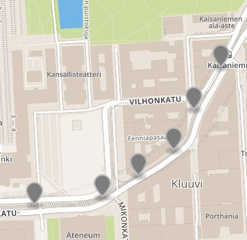
\includegraphics[width=0.45\textwidth]{screenshots/GPS_sample.png}
    }
  \quad
  \subfigure[GPS samples with noise]{
    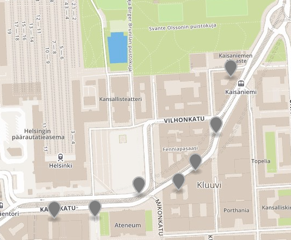
\includegraphics[width=0.45\textwidth]{screenshots/AfterBlur.png}
  }
  \caption{GPS Anonymization with Gaussian Noise}
  \label{fig:noise}
\end{figure}

\section{GPS Anonymization: K-Anonymity}
This method of GPS anonymization is a variant of Sweeney's K-Anonymity
\cite{sweeney2002k} applied to GPS data along the lines of Grutser and
Grunwald \cite{Gruteser2003}.  The basic idea is that the resulting
data from a single person should not distinguishable form data from
K-1 other persons. In order to achieve such kind of anonymization we
calculate for each GPS point $P$ by a user $U$ the $K-1$ nearest $GPS$
points $Q_1, \dots, Q_{K-1}$ which are recorded by $K-1$ different
users.  The anonymized point $R$ is now the centroid of the $K$ points
$(P,Q_1,\dots,Q_{K-1})$. This operations applied to all data points
$P$ in the dataset. The resulting anonymized points $R$ are stored in
a new table, so that these points do not take part in further the
centroid calculations.

Figure \ref{fig:k-ano} shows the results of application of K-anonymity
to the original GPS trip displayed in Figure \ref{fig:noise}.
$K$-Anonymity implementation script (cf. Figure \ref{fig:privacypy})
supports a second parameter that specifies the maximal distance that a
point can get displaced by this method.

\begin{figure}
  \centering
  \subfigure[K=7 anonymization]{
    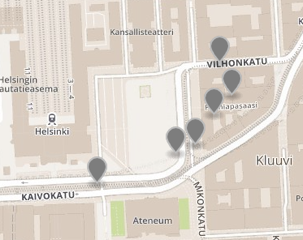
\includegraphics[width=0.4\textwidth]{screenshots/k_anon_7_nearest_points.png}
  }
  \quad
  \subfigure[K=15 Anonymization]{
    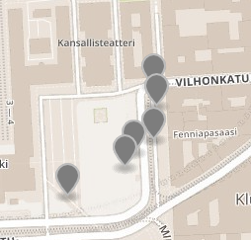
\includegraphics[width=0.4\textwidth]{screenshots/k_ano_15_nearest_points.png}
  }
  \caption{GPS Anonymization with K-Anonimity}
  \label{fig:k-ano}
\end{figure}

\section{GPS Anonymization: Haircut}

The \emph{haircut} anonymization method was developed by UKob to
address the problem of GPS tracks that show locations, like the home
address, that are unique to a single user. Looking on our data we see
many trips that originate at a unique location and later on meet other
tracks at locations of public interest like bus stops or larger
streets. The haircut methods cuts away parts of tracks that
"stick-out'' the whole set of recorded trajectories. For a given GPS
location $P$ the number of users is computed that have GPS samples
near to $P$. If this number is lower than a given threshold (e.g. $3$)
the point $P$ is dropped from the dataset.

The implementation script (cf. Figure \ref{fig:privacypy}) takes two
supports two parameters that specify the radius to look for other GPS
samples and the number of different users that are required to have
samples inside this radius. Figure \ref{fig:haircut} shows an example
a two-trips before and after the haircut.

\begin{figure}
  \centering
  \subfigure[Original GPS tracks]{
    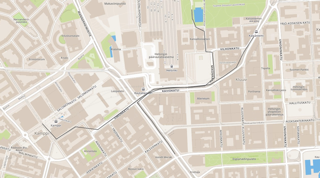
\includegraphics[width=0.4\textwidth]{screenshots/haircut_pre.png}
  }
  \quad
  \subfigure[GPS tracks with haircut]{
    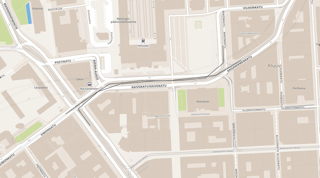
\includegraphics[width=0.4\textwidth]{screenshots/haircut_post.png}
  }
  \caption{GPS Anonymization with Haircut Method}
  \label{fig:haircut}
\end{figure}

